\documentclass[floatsintext, man]{apa6}
%\bibliography{references}
\usepackage{apacite}
\usepackage{subcaption}
\usepackage{booktabs}
\usepackage{xspace}
\usepackage[utf8]{inputenc}
\usepackage{amsmath}
\usepackage{amssymb}
\usepackage{tikz}
%\usepackage[sc,osf]{mathpazo}
\linespread{1.12}

% these packages are needed to insert results 
% obtained from R into the LaTeX document
\usepackage{pgfplotstable}
\usepackage{csvsimple}
\usepackage{siunitx}

% set the name of the folder in which the CSV files with 
% information from R is stored
\newcommand{\datafoldername}{csv_to_tex}


%\makeatletter
%    \let\@internalcite\cite
%    \def\cite{\def\citeauthoryear##1##2{##1, ##2}\@internalcite}
%    \def\shortcite{\def\citeauthoryear##1{##2}\@internalcite}
%    \def\@biblabel#1{\def\citeauthoryear##1##2{##1, ##2}[#1]\hfill}
%\makeatother


% the following code defines the convenience functions
% as described in the main text below

% rlgetvalue returns whatever is the in cell of the CSV file
% be it string or number; it does not format anything
\newcommand{\rlgetvalue}[4]{\csvreader[filter strcmp={\mykey}{#3},
             late after line = {{,}\ }, late after last line = {{}}]
            {\datafoldername/#1}{#2=\mykey,#4=\myvalue}{\myvalue}}

% rlgetvariable is a shortcut for a specific CSV file (myvars.csv) in which
% individual variables that do not belong to a larger chunk can be stored
\newcommand{\rlgetvariable}[1]{\csvreader[]{\datafoldername/myvars.csv}{#1=\myvar}{\myvar}\xspace}

% rlnum format a decimal number
\newcommand{\rlnum}[2]{\num[output-decimal-marker={.},
                             exponent-product = \cdot,
                             round-mode=places,
                             round-precision=#2,
                             group-digits=false]{#1}}

\newcommand{\rlnumsci}[2]{\num[output-decimal-marker={.},
                          scientific-notation = true,
                             exponent-product = \cdot,
                             round-mode=places,
                             round-precision=#2,
                             group-digits=false]{#1}}

\newcommand{\rlgetnum}[5]{\csvreader[filter strcmp={\mykey}{#3},
             late after line = {{,}\ }, late after last line = {{}}]
            {\datafoldername/#1}{#2=\mykey,#4=\myvalue}{\rlnum{\myvalue}{#5}}}

\newcommand{\rlgetnumsci}[5]{\csvreader[filter strcmp={\mykey}{#3},
             late after line = {{,}\ }, late after last line = {{}}]
            {\datafoldername/#1}{#2=\mykey,#4=\myvalue}{\rlnumsci{\myvalue}{#5}}}



\makeatletter
\patchcmd{\epigraph}{\@epitext{#1}}{\itshape\@epitext{#1}}{}{}
\makeatother \def\signed
#1{{\leavevmode\unskip\nobreak\hfil\penalty50\hskip2em
\hbox{}\nobreak\hfil#1% \parfillskip=0pt \finalhyphendemerits=0
\endgraf}} \newsavebox\mybox 

\newenvironment{aquote}[1]
{\savebox\mybox{#1}\begin{quote}} {\signed{\usebox\mybox}\end{quote}}

%\newcommand{\HRule}{\rule{\linewidth}{0.2mm}}



\title{Probabilistic Pragmatics in Syllogistic Reasoning}
\shorttitle{Pragmatics in Syllogistic Reasoning}

\author{Michael Henry Tessler\textsuperscript{1}\textsuperscript{,2}, Joshua B. Tenenbaum\textsuperscript{1}~\& Noah D. Goodman\textsuperscript{2}}
\date{}
  
\affiliation{
\vspace{0.5cm}
\textsuperscript{1} Department of Brain and Cognitive Sciences, Massachusetts Institute of Technology \\
\textsuperscript{2} Department of Psychology, Stanford University
}
%\authorsnames[{1,2},1,2]{Michael Henry Tessler, Joshua B. Tenenbaum, Noah D. Goodman}
%\authorsaffiliations{{Department of Brain and Cognitive Sciences, MIT}, {Department of Psychology, Stanford University}}

\date{}

\usepackage{xcolor}
\usepackage{bbm}

\newcommand{\denote}[1]{\mbox{ $[\![ #1 ]\!]$}}
\newcommand*\diff{\mathop{}\!\mathrm{d}}
\definecolor{Red}{RGB}{255,0,0}
\definecolor{Green}{RGB}{10,200,100}
\definecolor{Blue}{RGB}{10,100,200}

\newcommand{\mht}[1]{{\textcolor{Blue}{[mht: #1]}}}
\newcommand{\ndg}[1]{{\textcolor{Green}{[ndg: #1]}}}
\newcommand{\red}[1]{{\textcolor{Red}{#1}}}

\authornote{Corresponding author: Michael Henry Tessler, 450 Serra Mall, Building 420, Department of Psychology, Room 316, Stanford University, Stanford, CA 94305, USA. E-mail: tessler@mit.edu Present address: Department of Brain and Cognitive Sciences, Building 46, Room 3027,	Massachusetts Institute of Technology, 77 Massachusetts Avenue, Cambridge, MA 02139-4307, USA}

\abstract{\mht{abstract from 2014 cogsci paper}
Syllogistic reasoning lies at the intriguing intersection of natural and formal reasoning, of language and logic. Syllogisms comprise a formal system of reasoning yet use natural language quantifiers, and invite natural language conclusions. How can we make sense of the interplay between logic and language? We develop a computational-level theory that con- siders reasoning over concrete situations, constructed probabilistically by sampling. The base model can be enriched to consider the pragmatics of natural language arguments. The model predictions are compared with behavioral data from a recent meta-analysis. The flexibility of the model is then explored in a data set of syllogisms using the generalized quantifiers most and few. We conclude by relating our model to two extant theories of syllogistic reasoning – Mental Models and Probability Heuristics.}


\begin{document}
\maketitle


\begin{aquote}{\textbf{Walter J. Ong}, \emph{Orality and Literacy} (1982)}The syllogism is like a text: fixed, boxed-off, isolated... The riddle [by contrast] belongs in the oral world. To solve a riddle, canniness is needed: one draws on knowledge, often deeply subconscious, beyond the words themselves in the riddle. \end{aquote}

%\HRule

\section{Introduction}


Consider for a moment that your friend tells you: “Everyone in my office has the flu and, you know, some people with this flu are out for weeks.” You might respond: “I hope your officemates are not out for weeks and I hope you don’t get sick either.” The form of this exchange resembles a syllogism: a two- sentence argument used to relate two properties (or terms: A, C) via a middle term (B); the relations used in syllogisms are quantifiers. Fit into a formal syllogistic form, this argument would read:

All officemates are out with the flu (All A are B)

Some out with the flu are out for weeks (Some B are C) 

Therefore, some officemates are out for weeks (Some A are C)

Unfortunately, the conclusion does not follow from the premises (i.e., there is no relation between A \& C which is true in every situation in which the premises are true). Faced with such an argument, however, people are perfectly comfortable drawing some conclusion. A meta-analysis of syllogistic reasoning showed that over the population, the proper production of no valid conclusion responses for invalid arguments ranged from 76\% to 12\%. Even for valid arguments, the accuracy of producing valid conclusions ranged from 90\% to 1\% \cite{Khemlani2012}: people do not seem to find drawing deductively valid conclusions particularly automatic.

Many theories of syllogistic reasoning take deduction as a given and try to explain reasoning errors as a matter of noise during cognition. 
Errors, then, may arise from improper use of deductive rules \cite{rips1994, geurts2003reasoning} or biased construction of logical models \cite{JL1984, Newstead1992}. 
Many other kinds of reasoning, however, can be well-explained as probabilistic inference under uncertainty \cite{tenenbaum2006theory}. 
Probability theory provides a natural description of a world in which you don’t know exactly how many people are in your office are going to get the flu.

A separate dimension of theories of human reasoning concerns the extent to which principles of natural language — semantics and pragmatics — are necessary for understanding reasoning tasks. 
Natural language semantics plays a role in many such theories of reasoning \cite{JL1978, Khemlani2012, geurts2003reasoning}, though how issues of informativeness or relevance impact syllogistic reasoning either remain unclear \cite{Roberts2001} or are posited in an ad-hoc manner \cite{Chater1999}. 

In this paper, we explore the idea that the formalism of probabilistic pragmatics can provide insight into how people reason with syllogisms.
We present a model in the Rational Speech Act framework (Frank \& Goodman, 2012; Goodman \& Frank, 2016) that reasons about multiple quantifier sentences to produce a distribution over conclusions that follow from those sentences. We present three sets of results, highlighting the influence of different components of the model on human reasoning: (1) the influence of prior beliefs; (2) flexibility in natural language semantics, incorporating generalized quantifiers (e.g., “most” and “few”); and (3) pragmatic rea- soning. Previous approaches to the pragmatics of syllogistic reasoning have reduced the interpretations of syllogistic arguments to the interpretations of the individual premises or quantifiers used in those premises \cite{Roberts2001}. For example, premises involving the quantifier “some” may be interpreted as implying some but not all. But that sort of reasoning will not produce the conclusion in the syllogism above. Instead, what is needed is a richer scope of pragmatic reasoning: Reasoning about why about the speaker constructed the argument as a whole. We formalize this notion as a Question Under Discussion (C. Roberts, 2004) in which a listener reasons about the most likely conclusion (i.e., A–C relation) given the premises heard. We find that this formulation of pragmatic reasoning is able to break critical symmetries that would result from logical reasoning (Figure 1). An early version of this model was presented by Tessler and Goodman (2014).


%Cognitive theories of human reasoning turn along the critical dimension of whether the core ideal of reasoning is deductive validity or probabilistic support. 
%
%
%This cartoon illustrates a critical dimension along which cognitive theories of reason- ing differ: whether the core and ideal of reasoning is deduc- tive validity or probabilistic support. 
%
%
%An important extension to baseline CPT frameworks concerns incorporating pragmatics and language-like properties (such as compositionality) and representations in probabilistic inference. The probabilistic programming language (PPL) / probabilistic language of thought (PLoT) can more naturally apply to richer forms of reasoning, including everyday reasoning under uncertainty (e.g., Goodman et al., 2015). Furthermore, enriching these models with an understanding of natural language pragmatics can explain apparent fallacies in classical reasoning tasks (e.g., Tessler \& Goodman, 2014). Assuming a communicative context to a task involving language allows a reasoner in a PPL/PLoT model to incorporate the goals of a speaker (e.g., assuming the speaker intends to be informative), so providing a rational perspective on reasoning fallacies. We will also consider the way resource limitations guide practical models in PPL.
%
%
%
%
%By formalizing syllogistic reasoning as a probabilistic pragmatics problem, there is a natural way to account for influence of background knowledge in the form of the prior distribution on possible situations. We construct domains where we expect correlations between properties (e.g., knives – being sharp – cut well) and investigate syllogistic reasoning over these content domains. By measuring the prior probability of the eight possible combinations of binary features, we are able to generate predictions for syllogistic reasoning problems that are influenced by this kind of prior knowledge. Such influence of background knowledge on reasoning, known as belief bias in the syllogistic reasoning domain, has been of interest to psychologists for quite some time (e.g., Evans, Handley, \& Pollard, 1983; Dube, Rotello, \& Heit, 2010). We formalize this “bias” as rational belief updating given prior knowledge and find that the pragmatics model is too influenced by these kind of prior beliefs (Figure 2).





\section{Computational Model}





\section{Bayesian argument strength in syllogistic reasoning}

A formal account of gradience in syllogistic reasoning was presented by \citeA{Tessler2014}. The computational model is a Bayesian model; as such, it is important to understand the implications of the prior for syllogistic reasoning. I review the model, highlighting along the way how I generalize the model to consider content effects.

\subsection{Ontology}

The model is based on an ontology of situations represented by Venn diagrams corresponding to all possible logical relations between the sets of three properties (A, B, C). 

\begin{figure}[H]
\centering
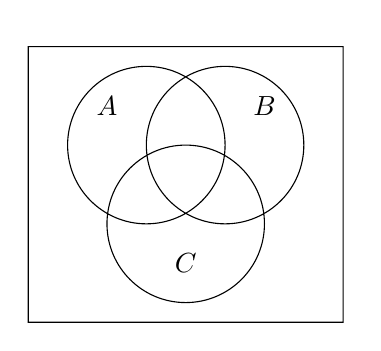
\begin{tikzpicture}[fill=gray]
% left hand
%\scope
%\clip (-2,-2) rectangle (2,2)
%      (1,0) circle (1);
%\fill (0,0) circle (1);
%\endscope
% right hand
%\scope
%\clip (-2,-2) rectangle (2,2)
%      (0,0) circle (1);
%\fill (1,0) circle (1);
%\endscope
% outline
\draw (0,0) circle (1) (-0.5,0.25)  node [text=black,above] {$A$}
      (1,0) circle (1) (1.5, 0.25)  node [text=black,above] {$B$}
      (0.5,-1) circle (1) (0.5,-1.25)  node [text=black,below] {$C$}
      (-1.5,-2.25) rectangle (2.5,1.25) node [text=black,above] {};
\end{tikzpicture}
\label{fig:venn}
\caption{Here is a caption.}
\end{figure}

Each Venn diagram is composed of 8 regions, corresponding to the presence or absence of each of the three properties: $\{\{A,B,C\}, \{A,B,\neg C\}, \{A,\neg B,C\}, \{\neg A, B, C\}, \{A, \neg B, \neg C\},...\}$. (For simplicity, we will refer to regions by the properties that are present, omitting the absent properties; for example, $\{A, B, \neg C\}$ will be referred to as $AB$.)
These regions can be thought of as unique object types (e.g., an object defined by having properties $A$ and $B$ but not $C$).\footnote{This diagram representation is analogous to a mental model in the style of \citeA{johnson1983mental} composed of object tokens (e.g., some objects which have properties $A$ or $B$, etc.) but where only unique object tokens are represented (e.g., there cannot be two objects which have the same set of properties).}
Then, a situation $s \in S$ is composed of the set of object types that are present.
For example, one situation could be $\{AB, BC, A\}$.
The set of unique situations (Venn diagrams) has size $2^8 = 256$, though we exclude the situation where all 8 regions are empty (i.e., there are no As, Bs, and Cs, but also no things that are not As, Bs, or Cs).

Situations $s \in S$ are probabilistically generated by sampling a Bernoulli random variable for each of the 8 regions. 

$$P(s) = \prod_{1\leq i\leq  8} P(A_{i}, B_{i}, C_{i}) $$%= (P(a) \cdot P(b) \cdot P(c)) ^n$$

%\subsection{Semantics}
The classical syllogisms are comprised by two premise arguments where each premise relates two properties via a quantifier. 
The quantifiers in classical syllogism are \emph{all}, \emph{some}, \emph{none}, and \emph{not all}.\footnote{
These quantifiers are typically presented in sentences such that \emph{none} is rendered as \emph{no} (e.g., No As are Bs) and \emph{not all} is rendered as \emph{some are not} (e.g., Some As are not Bs).
}
We use the classic logical semantics of these quantifiers: \emph{All As are Bs} entails that $\nexists (A \& \neg B)$;  \emph{Some As are Bs} entails that $\exists (A \& B)$; \emph{Some As are not Bs} entails that $\exists (A \& \neg B)$; \emph{No As are Bs} entails that $\nexists (A \& B)$.

\subsection{Argument strength}

The strength of a syllogistic argument (two premises) for a conclusion is a real-valued number between 0 and 1 given by the $P(u_c \mid u_1, u_2)$, where $u_1$ and $u_2$ are the two premises of the syllogism.
We compute this probability combining the prior distribution over situations with the literal meanings of the quantified statements: 

$$
P(u_3 \mid u_1, u_2) \propto \sum_s P(u_3\mid s) \cdot P(s \mid u_1, u_2)
$$

$$P(s \mid u_1, u_2) \propto P(s)\cdot \delta_{\denote{u_1}(s)} \cdot \delta_{\denote{u_2}(s)} $$


Truth-functional meanings of quantifier expressions are useful here because an expression which assigns a Boolean value to a situation can be used for probabilisitic conditioning. That is, these quantifier expressions can be used to update a prior belief distribution over situations into a posterior belief distribution: 
where $u_1, u_2$ are the two quantifier-utterances corresponding to the premises of a syllogism (e.g. $u_{\textrm{all  \emph{A} are \emph{B}}}, u_{\textrm{some  \emph{B} are not \emph{C}}}$).



To compute this probability, we first sample a situation and then evaluate wh




The truth conditions of the syllogistic sentences are determined by evaluating the object types that are present in a situation.


For syllogistic reasoning, we are interested not in the posterior distribution over situations \emph{per se}, but the distribution on true conclusions that these situations entail: $P(u_3 \mid s)$, where $u_3$ is a quantifier-utterance corresponding to the conclusion of a syllogism (e.g. $u_{\textrm{some  \emph{A} are \emph{C}}}$). Hence,




% For simplicity, we will refer to each region by the positive properties (i.e., properties which are present)
% In each situation, a region may be ``on'' or ``off'', corresponding to the presence or absence of that kind of object (e.g., if region "

% The set of unique situations (unique Venn diagrams) is $2^{3}$


composed of objects with properties, similar to mental models \cite{JL1983}. 
%
A situation $s \in S$ is composed of $n$ objects: $s = \{o_1, o_2, ..., o_n\}$, each of which can have 3 properties:
$$
s = \{ \{A_{o_{1}}, B_{o_{1}} , C_{o_{1}}\},  \{A_{o_{2}}, B_{o_{2}} , C_{o_{2}}\}, ... , \{A_{o_{n}}, B_{o_{n}} , C_{o_{n}}\} \}
$$

Properties $A$, $B$, and $C$ of these objects are stochastic
%but persistent\footnote{This is so a given object has the same value each time it is examined, even though that property-value is initially determined probabilistically} 
and assumed to be Boolean for simplicity. 
%
Properties \emph{across} objects are assumed to be independent and identically distributed \emph{(iid)}; hence, 
%\begin{align*}
%P(A_{o_{1}}, B_{o_{1}}, C_{o_{1}})			&					= P(A_{o_{i}}, B_{o_{i}}, C_{o_{i}}) \\
%			&					= P(a, b, c)
%\end{align*}
%and 
%
To account for syllogistic reasoning in \citeA{Chater1999}'s meta-analysis of 5 studies, which differed with respect to the materials used, the model assumed no \emph{a priori} information about the meaning of the properties; thus, properties  \emph{within} objects were determined independently and identically (\emph{i.i.d.}): $`$, with $p \sim \text{Bernoulli(}\theta\text{)}$.

The number of objects in a situation $n$ is a parameter of the model, as is the base rate $\theta$ of properties. In fitting the model to the meta-analysis data, \citeA{Tessler2014} found $\theta \approx 0.25$, qualitatively consistent with the ``rarity assumption''---that properties are relatively rare of objects---first used by \citeA{Oaksford1994}. The best fitting $n$ was around 5, also consistent with the ``minimal model assumption'' of the Mental Models framework \cite{JL1983}.


\subsection{A generative model of argument strength}

The generative model of situations can be turned into a generative model of syllogistic reasoning by providing a semantics for the quantifier sentences of a syllogism. The model uses the interpretation of quantifier sentences as truth-functional operators, consistent with standard practice in formal semantics. 

A quantifier utterance (e.g $u_{\textrm{all \emph{A} are \emph{B}}}$) maps two properties (e.g. \emph{A} and \emph{B}) to a truth value by consulting the properties of the objects in the situation $s$ and applying the usual literal meaning. For instance:
\begin{align*}
\denote{u_{\textrm{no  \emph{A} are \emph{B}}}}= \{s \in S : \| o_A \cap o_B \| = 0\}\\ 
\denote{u_{\textrm{some  \emph{A} are \emph{B}}}}= \{s \in S: \| o_A \cap o_B \|> 0\}\\
\denote{u_{\textrm{all  \emph{A} are \emph{B}}}}= \{s \in S: \| o_A \cap o_B \| = n\}\\
\denote{u_{\textrm{not all  \emph{A} are \emph{B}}}}= \{s \in S: \| o_A \cap o_B \|< n\}
\end{align*}
%
where $o_A = \{o_i | A_{o_{i}} = 1\} $ and $o_B = \{o_i | B_{o_{i}} = 1\} $ represent the objects in a situation that have the properties $A$ and $B$, respectively.
Thus, the quantifier utterances pick out the situations $s$ where the truth-functional meaning of the utterance is satisfied. 
 
Truth-functional meanings of quantifier expressions are useful here because an expression which assigns a Boolean value to a situation can be used for probabilisitic conditioning. That is, these quantifier expressions can be used to update a prior belief distribution over situations into a posterior belief distribution: 
$$P(s \mid u_1, u_2) \propto P(s)\cdot \delta_{\denote{u_1}(s)} \cdot \delta_{\denote{u_2}(s)} $$
where $u_1, u_2$ are the two quantifier-utterances corresponding to the premises of a syllogism (e.g. $u_{\textrm{all  \emph{A} are \emph{B}}}, u_{\textrm{some  \emph{B} are not \emph{C}}}$).

For syllogistic reasoning, we are interested not in the posterior distribution over situations \emph{per se}, but the distribution on true conclusions that these situations entail: $P(u_3 \mid s)$, where $u_3$ is a quantifier-utterance corresponding to the conclusion of a syllogism (e.g. $u_{\textrm{some  \emph{A} are \emph{C}}}$). Hence,

$$
P(u_3 \mid u_1, u_2) \propto P(u_3\mid s) \cdot P(s \mid u_1, u_2)
$$


This model, thus, returns a posterior distribution over conclusions conditioned on the premises of a syllogism being true.


The Bayesian model has a natural way of accounting for the influence of prior beliefs in reasoning. Indeed, beliefs simply specify a prior distribution over situations. In particular, the assumption that properties in a situation are independent and identically distributed \emph{(i.i.d.)} must be relaxed if we are to consider real-world content. I generalize the model by considering that properties can have correlations; the representation of expectations about the presence or absence of properties will be generalized from one marginal distribution---$P(p)=P(a)=P(b)=P(c)$---to the joint distribution: $P(a, b, c)$.



\section{Experiments}

\section{Discussion}


\newpage

\bibliographystyle{apacite}
\bibliography{syllogism}

\end{document}
